\documentclass{article}
\usepackage[utf8]{inputenc}
\usepackage{algorithm}
\usepackage{algpseudocode}
\usepackage{paracol}
\usepackage{amsmath}
\usepackage{amssymb}
\usepackage{bm}

\usepackage{setspace}
\onehalfspacing

\usepackage{geometry}
\geometry{margin=1.1in}



\setlength{\parindent}{0pt}
\setlength{\parskip}{1em}

\usepackage{amsmath,amsthm,amsfonts,amssymb,amscd, fancyhdr, color, comment, graphicx, environ}
\usepackage{float}
\usepackage{mathrsfs}
\usepackage{enumerate}
\usepackage[hidelinks]{hyperref}


\hypersetup{
    colorlinks=false,
    linkcolor=blue,
    filecolor=magenta,      
    urlcolor=blue,
    citecolor=black
}

\title{Thesis Draft}
\author{Lukas Gardberg}
\date{October 2022}

\DeclareMathOperator*{\argmax}{\arg\!\max}
\DeclareMathOperator*{\argmin}{\arg\!\min}

% Description of sections available in https://www.overleaf.com/project/633ee853c4abcf21aea5ca84
\begin{document}

\maketitle

\newpage

\section{Abstract}

\newpage

\tableofcontents

\newpage

\section{Introduction}

% Ta evenutellt inspiration från hifi-gan introduction

In recent years, the amount which humans utilize software systems for communication has increased significantly. Ranging from the early beginnings of email, text messaging, and cellular calls, to modern voice and video chats through mobile applications. However, as these technologies have progressed, so has our ability to automate parts of the interaction. Be it pre-recorded messages, selecting an option on your keypad, or automatically generating responses to emails.

One such area of innovation is spoken conversation, where modern communication software strives to make the interaction personal by developing systems that are adaptable with regards to the human on the receiving end. Such a system needs to be able to understand the chosen medium, interpret what the human is communicating, and respond appropriately. This entails a level of natural language understanding, the ability to generate a natural sounding spoken response, and is an active research area.

Efforts have historically aimed to mimic the biological systems which give rise to speech in humans, either mechanically \cite{von1791mechanismus}, or through formant synthesis and vocal chord modelling \cite{fant1970acoustic}. Significant progress has also been made using rule- and expert-based systems which incorporate knowledge from experts (such as linguistis) in order to achieve natural speech \cite{klatt1980software}. In addition to this, concatenative speech synthesis has also produced promising results, and is based on stitching together pre-recorded audio clips in order to obtain a target pronunciation. However, all of these methods exhibit several drawbacks, e.g. in the form of limited flexibility, heavy reliance on human knowledge, and varying naturalness of speech \cite{tan2021survey}.

In order to overcome these challenges the use of statistical parametric speech synthesis (SPSS) has grown, which aims to model the varying processes in speech using parametrized models and large amounts of data. This approach is usually divided up into three steps: text analysis, parameter prediction (acoustic model), and synthesis (vocoder). The first step involves processing the text to be spoken, which includes e.g. normalization, segmentation, and phoneme conversion, which gives more detail to the pronunciation of the text. Secondly an acoustic model is tasked with generating computer processable acoustic features, which can be seen as a compact representation of the characteristics of the audio. Examples include fundamental frequencies and spectra. Lastly a vocoder model generates audio (e.g. an audio file) based on prior acoustic features \cite{zen2009statistical, tan2021survey}. 
% Image adopted from \cite{tan2021survey}.
\begin{figure}[H]
    \centering
    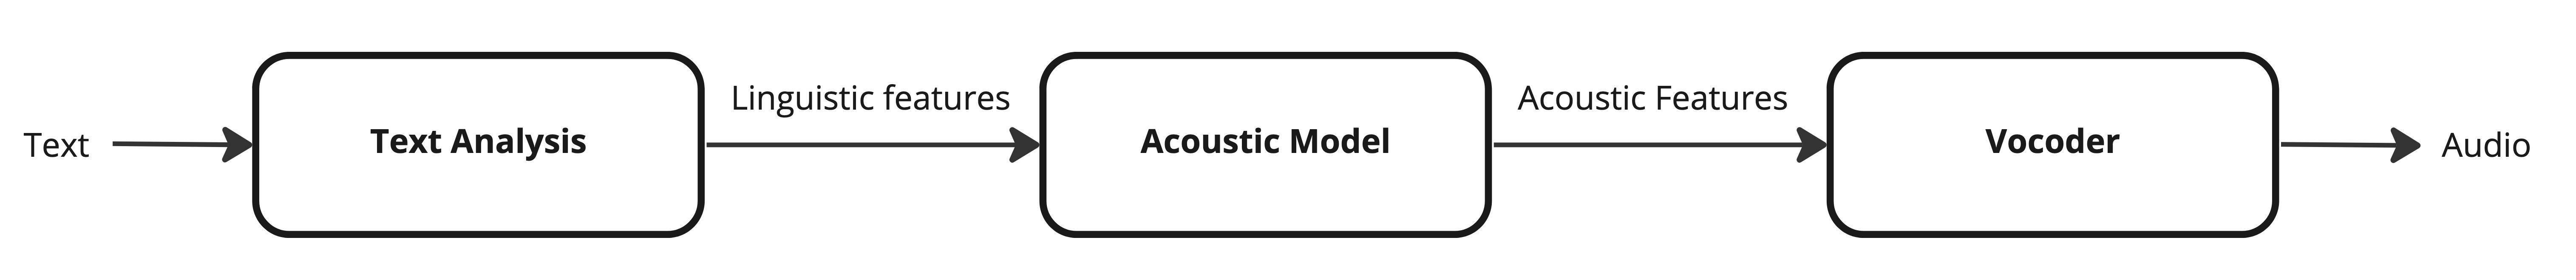
\includegraphics[scale=0.07]{images/TTS.jpeg}
    \caption{\onehalfspacing Schematic overview of common text-to-speech components. The input text which speech is to be generated for is first analyzed to produce linguistic features. These are then fed into an acoustic model outputting acoustic features, e.g. a mel spectrogram. Lastly the acoustic features are converted into audio using a vocoder model.}
    \label{fig:TTS}
\end{figure}
Many of these ideas persisted in tandem with the rise of deep learning and the utilization of increased computational power. Neural networks have thus successfully been incorporated into all stages of SPSS \cite{ze2013statistical, arik2017deep}, and research has since moved towards a fuller end-to-end approach \cite{oord2016wavenet} which has seen great success in several other areas  \cite{krizhevsky2017imagenet, bojarski2016end, zhou2018voxelnet}. This has popularized the term \textit{neural TTS}, where the fully end-to-end refers to the task of generating speech directly from text, using no direct intermediate representations.

This thesis focuses on the last step of the process, the \textit{vocoder}, and the challenges of incorporating a neural network-based vocoder into a user-facing application. Special weight is put on \textit{diffusion-based} vocoders, which is a specific type of machine learning model which has shown great promise in several other areas. 

\subsection{Previous work}
%(Var passar denna del in? Antar en del förkunskap om NNs)
The first vocoder based on neural networks is WaveNet which was proposed in 2016 \cite{oord2016wavenet}. Contrary to spectrograms it uses linguistic features directly as inputs in order to generate audio on the sample level. It is also autoregressive, meaning that each sample is conditioned on all previous ones, and that audio therefore is generated in a circular fashion by feeding in past outputs to the input. The backbone of WaveNet is the 1-D causal convolution layer, which provides learnable filters applied only on past samples relative to the current one. In addition to this, dilation is also leveraged in order to provide the filters with a wider receptive field and achieve greater efficiency. It is worth noting that one of the main drawbacks of WaveNet and similar autoregressive models is that waveform generation is not parallelizable, therefore resulting in a longer inference time via the inherent sequential nature. Several efforts have been made in order to reduce the inference, for example through pruning or caching \cite{kalchbrenner2018efficient, paine2016fast}.

Later progress involved developing a fuller end-to-end sequence-to-sequence approach with Tacotron \cite{wang2017tacotron} and Tacotron 2 \cite{shen2018natural}. The proposed encoder in the first version addressed the limitations of using complex linguistic features, and instead aimed for a transformer-based model which produces mel spectrograms from character sequences. The vocoder part involved simple Griffin-Lim reconstruction, and was later improved in the second iteration. The improvement consisted of replacing the non-parametric vocoder with a WaveNet-based neural network which could be trained separately to the encoder to produce audio from mel spectrograms.

Following the advancement of using a neural network-based vocoder, several different directions have been taken. One of the main problems addressed is creating a non auto-regressive model, and speeding up inference through parallelizable architectures. One such family of models used as vocoders are \textit{flow-based} models. These utilize a normalizing flow which iteratively transforms a simple distribution into a complex one (i.e. the distribution of speech data) using a series of invertible mappings, and can thus achieve an approximation of a target posterior distribution \cite{rezende2015variational}. For example, WaveGlow \cite{prenger2019waveglow} is a flow-based vocoder which combines progress from Glow \cite{kingma2018glow} and WaveNet to non-autoregressively generate audio above 16kHz faster than real-time. 
%Interestingly, there are several similarities with denoising diffusion probabilistic models. Most notable is the iterative nature of the computations, and the idea of starting with a simple distribution, such as a unit Gaussian and sequentially obtaining a more complicated one.

In addition to this, generative adversarial networks (GANs) have also been utilized as vocoders \cite{goodfellow2020generative}. The principle behind a GAN is to jointly train a generator network to generate samples from noise, and a discriminator network to determine if a candidate sample is real or synthesized. Examples include WaveGAN \cite{donahue2018adversarial} which relies on a deep convolutional neural network as the generator, and improvements such as GAN-TTS \cite{binkowski2019high}, and HiFi-GAN \cite{kong2020hifi} which leverage techniques such as multiple discriminators and augmented loss functions. Such models are able to generate high fidelity audio effectively using only a single forward pass, but have been shown experimentally to be difficult to train (e.g. mode collapse) and are not able to produce likelihood estimates as a consequence of the architecture. However, they are widely considered to be the state-of-the-art in terms of inference speed.

The main model considered in this thesis is DiffWave \cite{kong2020diffwave}, which is the first diffusion-based vocoder, characterized by it's audio-specific architecture and conditioning on spectrograms generated by an acoustic model. The model is decribed in further detail in section \ref{sec:diffvoc}.

\subsection{Problem statement}

The goal of this thesis is to explore the usage of denoising diffusion probablilistic models as vocoders, what aspects are favorable or limiting in real-time applications, and how they compare to other current machine learning-based models for speech generation. To achieve this, the aim is to answer three main questions:

(TODO: Refine further)

\begin{itemize}
    \item What are the strengths and weaknesses of denoising diffusion probabilistic models in general?
    \item How do suggested model improvements from other domains affect performance in the vocoding task?
    \item Can diffusion based vocoders be used in real-time text-to-speech applications?
\end{itemize}

\newpage
\section{Theory}

This section introduces the major theoretical building blocks needed to understand diffusion models, as well as tools and techniques related to the vocoder problem. The processing and analysis of audio signals is covered, including the three different waveform-, spectrogram-, and mel spectrogram-representations. In addition to this, a brief introduction to machine learning and learning algorithms is given in order to provide context for the modelling and optimization methods used. Lastly the diffusion framework is presented along with current limitations and challenges, as well as a discussion on suitable evaluation methods for generative models.

\subsection{Sound \& Signals} \label{sec:sounds}

The natural representation of a sound, and what our human ears have evolved to perceive, is a repetitive increase and decrease in air pressure in the form of an acoustic wave. The source of a wave can for example be a vibrating membrane whose movement sets air into motion, such as our vocal chords. Each sound possesses a certain \textit{frequency} representing how many times the acoustic wave compresses and de-compresses (oscillates) per unit of time, and is measured in Hertz (Hz). Humans have evolved to perceive sounds with a frequency between 20 Hz and 20 kHz, where sounds outside of this range are inaudible to us. Sound is most commonly recorded via a microphone in which a fixture is displaced by the propagating wave. The component inside the microphone is configured to induce an electrical signal representing the movement of the air.

In order to represent such an analog signal digitally, its value (the amount of voltage or current) is measured at a certain rate, i.e. \textit{sampled}, where the discrete measurements are represented using quantized amplitude values such as floating point units. The rate at which the signal is measured is called the \textit{sample rate} $f_s$ (Hz). As a consequence of the Nyquist-Shannon sampling theorem a digital signal can only represent an analog signal without distortion (aliasing) if it is sampled with a sample rate at least double the frequency of the highest frequency in the analog signal. For example, a signal sampled at 44 100 Hz can at most adequately represent an analog signal of 22 050 Hz, making it an appropriate sample rate for human hearing. (Cite?)

Mathematically it is possible to represent an audio signal in several ways. One form suitable for theoretical analysis is to define it as a function $x: \mathbb{R} \rightarrow \mathbb{R}$, where $x(t)$ represents its amplitude at a real valued time-point $t \in \mathbb{R}$. However, in practice measured signals are not defined at infinitely many points, but are rather of limited size as a consequence of the time interval over which they were sampled being finite. We define such a real-word signal as a \textit{vector} $\bm{x} = [x[0], \, \dots, \, x[L-1]]^{\text{T}} \in \mathbb{R}^{L}$ which consists of $L$ real-valued amplitude samples indexed from $0$.

\subsubsection{The Short-time Fourier Transform} \label{sec:stft}

For the task of analyzing the frequency contents of signals such as audio, the \textit{Fourier Transform} is a common and useful tool. Given a signal $x: \mathbb{R} \to \mathbb{R}$ its transform $y: \mathbb{R} \to \mathbb{C}$ is defined as
\begin{equation}
\label{eq:fouriert}
    y(f) = \int_{-\infty}^{\infty} x(t) e^{-i 2\pi f t} \, dt,
\end{equation}
for a specific frequency $f\in\mathbb{R}$. The resulting function $y$ provides amplitude and phase information of each frequency contained in $x$ in the form of the absolute value and the argument of the resulting complex number. Intuitively the Fourier Transform can be interpreted as a measure of how correlated a signal is with a sinusoid of frequency $f$. Once $y$ has been obtained, it is also possible to perform an inverse transform
\begin{equation}
    x(t) = \int_{-\infty}^{\infty} y(f) e^{i 2\pi f t} \, df
\end{equation}
in order to recover the original signal $x$ under certain conditions.

As earlier described, signals are often represented as sampled values at discrete time points in contrast to a real valued function. The respective transform for a discrete-time signal $\bm{x}=\left[ x[0], x[1], \dots , x[L-1] \right]^{\text{T}}$ is the \textit{Discrete Fourier transform} (DFT), which is defined as
\begin{equation}
    y[k] = \sum_{n=0}^{L-1} x[n] e^{-i \frac{2\pi}{L}k n},
\end{equation}
resulting in a new complex valued vector $\bm{y} = [y[0],\dots, y[L-1]]^{\text{T}}$ where $\bm{y}\in \mathbb{C}^{L}$. Worth noting is that both these transforms analyze the complete signal all at once which yields a static spectrum, and can thus be ill suited for signals whose frequency content change over time. An example of such a changing signal is recorded speech, where the pronunciation of different vowels and consonants in the form of sustained and plosive sounds result in a dynamic frequency distribution.

In order to account for this variability the signal can instead be analyzed at several overlapping individual segments. This is done by \textit{windowing} the signal with a window function $w$ which is zero outside of a set width. In practice this function is represented as a vector $\bm{w}=[w[0],\dots, w[L-1]] \in \mathbb{R}^L$. The resulting transform of such a windowed signal gives a representation of the frequency content of that particular segment, allowing several such windowed transforms to be combined into a time-dependent frequency distribution. This process is performed using the \textit{Short-time Fourier Transform} (STFT), which for a signal $\bm{x}$ and window function $\bm{w}$ is defined as
\begin{equation}
    \text{STFT}\left\{ \bm{x} \right\}(k, m) = Y[k, m] = \sum_{n=0}^{N-1} x[n]w[n+mH]e^{-i \frac{2\pi}{N}k n}.
\end{equation}
Here $k$ represents the frequency bin index, and $m$ the time frame index. The \textit{hop length} of the window is denoted by $H$ which determines the distance between two adjacent windows. Note also that the number of evaluation points $N \leq L$ have to be chosen, which differs from the number of samples $L$ in $\bm{x}$. The result of the STFT is a matrix $\bm{Y} \in \mathbb{C}^{K \times M}$ of complex numbers $Y[k, m]$ for each frequency and time index. However, this representation is impractical for humans to analyze manually through e.g. visual inspection. One approach of reducing the complexity and obtaining a visual representation is to calculate the \textit{spectrogram} $\bm{S}$, which is defined as the element-wise squared magnitude of the STFT matrix $\bm{Y}$, i.e.
\begin{equation}
    S[k, m] = \left| Y[k, m] \right|^2.
\end{equation}
Each resulting element $S[k, m]$ is thus a real value, which enables $\bm{Y}$ to be displayed as an image. One important aspect of this simplification is that when the entries of the complex matrix $\bm{Y}$ are squared, some phase information of the signal is lost (the arguments of the complex numbers), and a lossless inverse transform is no longer possible. This leaves the power spectral density, which can be seen as a representation of how the energy is divided between the different frequencies over time. An example of a speech recording and its spectrogram can be seen in figure \ref{fig:melspec}.

\begin{figure}[H]
    \centering
    \includegraphics[scale=0.5]{images/melspec.png}
    \caption{\onehalfspacing Waveform, Spectrogram, and Mel Spectrogram representation of the spoken sentence \textit{"In good printing, the spaces between words should be as near as possible equal"}. The $x$-axis denotes the time in seconds, and the $y$-axis denotes the frequency- and mel-bins for the spectrogram and mel spectrogram respectively. Note that the mel spectrogram contains fewer bins than the spectrogram as a result of the choice of 80 mel filters, but that we observe a more detailed resolution for the speech components of the signal in the form of overtones. A brighter point represents a larger magnitude. Spectrograms were obtained identically as described in section x.}
    \label{fig:melspec}
\end{figure}

One notable aspect of the STFT is that the resolution of $\bm{Y}$ in both time and frequency is related to the choice of window $\bm{w}$. For a wider window a greater frequency resolution is achieved, meaning that it becomes easier to distinguish between components which are close in frequency. However, a wider window results in worse time resolution, as fewer windows are needed to cover the entire signal. Conversely a narrow window gives better time resolution as the DFT is calculated at more time steps, but a worse frequency resolution. This trade off makes the choice of $\bm{w}$ important, and has given rise to  several methods which aim to analyze the signal at multiple time- and frequency resolutions. (cite?)

TODO: Add MFCC definition

\subsubsection{The Mel Spectrogram} \label{sec:melspec}
When analyzing a signal using the STFT the resulting complex matrix $\bm{Y}$ contains information about its frequency content for each \textit{linearly spaced} frequency $k$. However, it is widely understood that the human perception of the distance between two different frequencies is not linear, as experiments have shown that this distance gets larger for higher frequencies \cite{stevens1937scale}. This is characterized by the \textit{mel-scale}, which can be used to transform a linear frequency scale into one that is adjusted for human hearing. Transforming a spectrogram according to this scale results in a \textit{mel spectrogram}, and provides a higher frequency resolution for the range of frequencies in which human speech is centred. Such a transform which maps a frequency $f$ in Hertz into \textit{mels} is defined as
\begin{equation}
    f \longmapsto 2595 \log_{10} \left( 1 + \frac{f}{700} \right).
\end{equation}
Also worth noting is that the transform compresses higher frequencies and expands lower ones through it's logarithmic transform. This can also be seen as a representation which is closer to how the brain processes sound, and is thus better suited for representing human speech.

In practice a mel spectrogram is obtained using a mel-frequency filter bank. For each time step in the spectrogram, each mel coefficient is obtained by multiplying the corresponding spectrum with a band-pass filter, such as a triangle window. For e.g. 80 filters this results in 80 mel components, corresponding to the $y$-axis of the mel spectrogram in figure \ref{fig:melspec}. The band-pass filters are chosen to be \textit{linearly spaced in the mel-scale}, meaning that frequencies are equal distances apart in terms of how they are perceived by humans. The process of transforming a magnitude spectrogram $\bm{S}$ of size $K \times M$ into a mel spectrogram $\bm{S}_{\text{mel}}$ of size $K_{\text{mel}} \times M_{\text{mel}}$ can be defined as $\mathcal{M}: \bm{S} \mapsto \bm{S}_{\text{mel}}$. An example of a mel spectrogram can be seen in figure \ref{fig:melspec}, and for the specific mel spectrogram settings used in experiments, see section x.

Overall the mel spectrogram provides a natural way of representing human speech in a format which is processable by computers. Importantly it is a more compressed representation of the audio. For example, the waveform in figure \ref{fig:melspec} contains around 120 000 samples, while the corresponding mel spectrogram shown only contains around 38 000, which is roughly three times as few. In practice the actual size in memory would depend on other aspects such as floating points precision, but it nonetheless highlights one of the main favourable qualities of the representation.

\subsubsection{Phase Reconstruction Problem} \label{sec:phaseprob}

Say a spectrogram representation of a signal has been obtained, but the original signal is no longer available. How would one go about recreating the original signal? This is called the \textit{phase reconstruction problem}, which refers to the fact that if the original phase of the signal is reconstructed the signal can easily be recovered through an inverse transform. As described in sections \ref{sec:stft} and \ref{sec:melspec}, signal information is discarded both in the complex- to real-valued spectrogram computation, as well as the mel-frequency filter bank transformation. Considering the problem of recovering a signal $\bm{x}$ from its mel spectrogram, the mel spectrogram is first obtained through an STFT, a magnitude transform, and a transform $\mathcal{M}$. The heart of the phase reconstruction problem lies in being able to invert this process using a \textit{vocoder} in order to recover a signal $\tilde{\bm{x}} \approx \bm{x}$. This series of transformations is depicted in figure \ref{fig:phasere}. Note that a mel spectrogram is obtained directly from the available ground truth signal when training the vocoder, whereas during inference for text-to-speech it would be provided by an acoustic model as in figure \ref{fig:TTS}.

\begin{figure}[H]
    \centering
    \includegraphics[scale=0.15]{images/Phase_reconstruction.png}
    \caption{\onehalfspacing The process of obtaining a mel spectrogram $\bm{S}_{\text{mel}}$ from an original signal $\bm{x}$, and recreating it using a vocoder. The signal is first transformed using a Short-time Fourier Transform, which is depicted using a bidirectional arrow to emphasize its invertibility. A spectrogram $\bm{S}$ is then obtained though a magnitude transform, followed by a mel spectrogram $\bm{S}_{\text{mel}}$ via a transform $\mathcal{M}$. These transforms are shown as unidirectional since they are non-invertible. Lastly the vocoder performs the inverse mapping to obtain $\tilde{\bm{x}}$. This procedure is followed during training of the vocoder model in order to generate training data, whereas during inference the mel spectrogram is generated by an acoustic model.}
    \label{fig:phasere}
\end{figure}

At a first glance modelling such a transformation may seem impossible through a lack of information. However, previous research has shown both experimentally and theoretically that the problem is tractable by e.g. utilizing a number of underlying connections between the phase and the magnitude of the spectrogram, or learning the mapping via large amounts of data \cite{kawahara1999restructuring, agiomyrgiannakis2015vocaine, hayes1980signal, auger2012phase}. (Lägga till något om att träna på spectrogram genererade från ground truth data vs från en acoustic model?)

Historically there have been many different approaches to solving the phase reconstruction problem. It is evidently of special interest for text-to-speech applications because of the need to transform the acoustic features generated by an acoustic model into audio. The main focus in this thesis is on learning the inverse mapping needed for reconstruction through a statistical model trained on a large amounts of mel spectrogram and audio pairs. However, popular preceding methods were often data-agnostic and instead exclusively relied on numerical optimization or instrinsic assumptions about the signal, which here can be of great use as a baseline \cite{toda2007voice, griffin1984signal}.

% As for many generative modelling tasks, obtaining an objective metric which effectively represents human-perceived quality is a challenge. Traditionally, previous studies have mainly used a mean opinion score (MOS), which consists of a mean rating of samples generated from e.g. test set given by a group of human evaluators. Obtaining these can however be a costly process, which have led to the use of several quantitative metrics which aim to approximate such a qualitative score. The chosen quantitative metrics are described in the following sections.

\subsubsection{Griffin-Lim reconstruction}

The Griffin-Lim vocoder is a traditional approach used to recover an audio signal from the magnitude of its STFT. More specifically, it is based on reducing a simple mean squared error between the magnitude of the STFT of the estimated signal $\tilde{\bm{x}}$ and the original magnitude representation, i.e the spectrogram. The number of iterations can manually be adjusted to achieve a better reconstruction. The algorithm was originally proposed in 1984, has since then been used as a baseline in several previous vocoder studies \cite{wang2017tacotron, prenger2019waveglow}, and provides a simple and non-parametric way of solving the phase reconstruction problem \cite{griffin1984signal, albadawy2022vocbench}.

\subsection{Learning Paradigms \& Generative Models}

Some of the first attempts to solve the phase reconstruction problem consisted of methods which mainly relied on signal assumptions and numerical optimization, and more importantly only considered a single signal at a time. The alternative emergent approach is to instead attempt to learn the mapping by using information from a large amount of samples in the hope of achieving a solution which performs better in general. The process of creating a statistical model to solve a task by observing data is one way to define \textit{machine learning}. It has become especially prominent today thanks to more data being readily available, and an increased capability of performing large-scale computation, especially in parallel.

Historically the most common learning framework is \textit{supervised learning}. Given a set of pairs of samples (e.g. audio signals) $\bm{x} \sim q$ drawn from a data distribution $q$ and labels $y$, the goal is to learn the probability of a sample $\bm{x}$ having label $y$, i.e. $q(y\mid \bm{x})$. The term "supervised" is used because the ground truth label $y$ needs to be assigned by a human, essentially \textit{supervising} the learning. Because the data of interest often times is high dimensional and possesses a complex structure it is impossible to obtain $q(y \mid \bm{x})$ explicitly. Therefore an approximate model $q_{\theta}(y \mid \bm{x})$ is used to estimate $q(y \mid \bm{x})$, where $\theta$ are the parameters defining the model to be learned. A common goal of supervised learning is to be able to classify samples $\bm{x}$ into one of several categories, such as if an image represents a cat or a dog, or if an audio recording consists of a dog barking or a cat meowing \cite{goodfellow2016deep}. 

Related is the task of \textit{unsupervised learning} which aims to approximate the original underlying data distribution $q(\bm{x})$ which the observed data stems from. This is similarly done through an approximate model $q_{\theta}(\bm{x})$ which estimates $q(\bm{x})$. The goal of unsupervised learning is often to be able to generate new, unseen samples from $q(\bm{x})$ using $q_{\theta}(\bm{x})$, and is the specific sub-field especially considered in this thesis, coined \textit{generative models}. In certain cases it may be desirable to obtain explicit probability values $q(\bm{x})$, e.g. for comparing the negative log likelihood between models (see section \ref{sec:learn}). However, in the context of generative models weight is rather put on being able to generate new "realistic" samples which follow the original probability distribution as closely as possible, allowing $q(\bm{x})$ to only be available implicitly \cite{foster2019generative}. Evaluating such a model without access to $q(\bm{x})$ is further discussed in section \ref{sec:eval}.

Closely tied to unsupervised learning is \textit{self-supervised learning}. Instead of using a human-made learning signal $y$, a model is trained by withholding some information from the data, which then is to be predicted using the remaining available data. In this way the learning signal instead comes directly from the data set, which is why the model can be considered to supervise itself. For example, both language models and speech recognition systems can be trained through \textit{input masking} where the model is tasked with predicting a removed part of a sequence given the preceding data, such as a sentence or a waveform. However, there is not a clear boundary between self-supervised and unsupervised learning, and the chosen vocoder model framework can therefore both be considered to be unsupervised and self-supervised \cite{baevski2020wav2vec, devlin2018bert}.

In the case when labels $y$ exist, it is also possible to create a generative model which estimates $q(\bm{x} \mid y)$, i.e. conditions on the label. In the case of generating cat and dog sounds, one could imagine the model to be conditioned to either generate audio of a dog or a cat by feeding the label into the model during sample generation. The idea of learning both tasks jointly and guiding the sample generation via a label is that the model can learn patterns common to both tasks. In practice the information a generative model is conditioned on does not have to be a label or a category, and can just as well be any other type of data which provides the model with an informative signal which limits the range of data considered. In the context of vocoders and the phase reconstruction problem, the vocoder is conditioned on acoustic features such as a mel spectrogram when performing the task of generating speech, which one can imagine limits the number of plausible audio sources significantly.


\subsubsection{Neural Networks}

In order to obtain a good enough approximation $q_{\theta}(\bm{x}) \approx q(\bm{x})$ the first step is to choose a function $q_{\theta}$ which is able to capture the complexity of $q$ adequately. For example, if we know that $\bm{x}$ is drawn from a normal distribution, i.e. $q(\bm{x}) = \mathcal{N}(\bm{x} \mid \bm{\mu}, \bm{\sigma}^2)$ it is reasonable to choose a model $q_{\theta}(\bm{x}) = \mathcal{N}(\bm{x} \mid \bm{\mu}_{\theta}, \bm{\sigma}_{\theta}^2)$. In fact in this case one can show that we can obtain an approximation which is arbitrarily close to $q$ with enough data (cite?). However, that is not true for any type of distribution $q$, and it becomes significantly harder to come up with or even reason about what type of distribution a sample stems from when the data is more complex. Loosely speaking, we can say that the \textit{capacity} of the chosen model $q_{\theta}$ is limited since it is restricted to modelling normally distributed data. Conversely we would say that a model which can capture more complex data distributions, i.e. approximate more complex functions, has a higher capacity. One model with such capability is the \textit{neural network}.

A neural network consists of a combined number of functions which are chained together to produce an output. The main idea is to obtain a function with higher capacity by combining several non-linear functions with lower capacity. One such basic function is the perceptron. Given an input vector $\bm{x}=[x_0, \dots, x_{L-1}]^\text{T}$, which e.g. can represent an audio signal where each element $x_k = x[k]$ (as defined in section \ref{sec:sounds}), a perceptron takes one or more inputs $x_k$, performs an affine transformation, and then passes the combined value through an element-wise non linear \textit{activation function} $\varphi$. A perceptron $k$ is parametrized by its multiplicative weights $\bm{w}_k$ and additive bias $b_k$. The output $h_k$ can be written as
\begin{equation} \label{eq:perc}
    h_k = \varphi\left( \bm{w}^T_k \bm{x} + b_k \right), \ \ \theta = \{ \bm{w}_k, b_k\}.
\end{equation}
Several of these perceptrons can be stacked and their output combined in order to form a \textit{layer}, where the number of perceptrons in the layer is called the \textit{width}. The layer will then have an output for each perceptron, which can be written in vector form as
\begin{equation}
    \bm{h} = \varphi\left( \bm{W}^T \bm{x} + \bm{b}\right), \ \ \theta = \{ \bm{W}, \bm{b} \},
\end{equation}
where each perceptron in the layer takes in all inputs $\bm{x}$ from the previous layer, making it fully connected. Here $\bm{W}$ is an $L \times P$-matrix, where $P$ is the number of outputs $h_k$, where each row $k$ represents the multiplicative weights of perceptron $k$. The output $\bm{h}$ and bias $\bm{b}$ are both column vectors of length $P$. For example, the outputs of the "hidden layer" $\bm{h}$ of the network shown in figure \ref{fig:NN} is calculated as
\begin{equation}
\underbrace{
\left[
    \begin{array}{c}
         h_0 \\
         h_1 \\
         h_2
    \end{array} \right]}_{\bm{h}}
= \varphi \left(
\underbrace{\left[ \begin{array}{cc}
     w_{0,0} & w_{0,1} \\
     w_{1,0} & w_{1,1} \\
     w_{2,0} & w_{2,1}
\end{array} \right]}_{\bm{W}^T}
\underbrace{
\left[ 
\begin{array}{c}
     x_0  \\
     x_1 
\end{array}
\right]}_{\bm{x}} +
\underbrace{\left[ 
\begin{array}{c}
    b_0 \\
    b_1 \\
    b_2
\end{array}
\right]}_{\bm{b}}
\right),
\end{equation}
where $w_{k,j}$ corresponds to the weight of perceptron $k$ on input component $j$. Consequently it is possible to both extend the neural network by increasing the width of the hidden layer, or adding more hidden layers (i.e. increasing the depth). Both the depth and width extension provide the network with more learnable parameters, and thus increase its capacity. Creating such a network with several layers is often called a \textit{multilayer perceptron} (MLP) and can be considered the cornerstone of the field \textit{deep learning}, which deals with MLPs of considerable depth.

When training such a network the dimensionality of the input is often decreased with the depth as a consequence of the architecture. This results in the network being forced to achieve more effective representations of the input data if it is to succeed at the task its being train to perform (commonly identified as \textit{representation learning}). These intermediate lower-dimensional representations are often called \textit{embeddings}, and can in fact be used to perform other tasks as well. For example, a language model might have been trained in a self-supervised fashion to generate text, and through this learned to generate effective text embeddings. These can then be utilized to e.g. classify text by using them as inputs to another model.

The neural network or MLP architecture provides an effective way to adjust the capacity of our approximating function. In fact it has been shown that neural networks are universal approximators, meaning that they can approximate (almost) any function or probability distribution arbitrarily well provided either unlimited depth or width \cite{hornik1989multilayer, lu2020universal}. This flexibility is one of the main reasons for their widespread usage. However, the process of actually obtaining such an approximation is an entire challenge of its own, and has arguably been one the main areas of research focus within the field in recent years.


\begin{figure}[H]
    \centering
    \includegraphics[scale=0.3]{images/NN.png}
    \caption{\onehalfspacing A depiction of a simple neural network with two inputs, a single hidden layer with a width of three, and a single output. Each hidden value $h_k$ is calculated via equation (\ref{eq:perc}). The right side of the figure shows the network written in vector form.}
    \label{fig:NN}
\end{figure}

Even though the "vanilla" neural network architecture can in theory approximate almost any function, doing so effectively using a limited number of weights is hard, as well as obtaining an approximation which generalizes to unseen data. One approach of easing the learning process is to adapt its architecture to the modality of the data. This has for example been done for images via the \textit{convolutional neural network} (CNN) \cite{lecun1989backpropagation}. Its structure is based on the assumption that the relationship between samples (e.g. pixels) is highly local, and thus only considers a subset of the input at a time compared to regular fully connected networks. This subset is often times in the form of a filter which is moved across the signal and used to calculate an element-wise product at each position. In the image case the filter can be of shape $D \times H \times W$, where $D, H$ and $W$ represent the size of the depth, height, and width of the filter. For a one dimensional signal it usually of the shape $1 \times F$, where $F$ represents the length of the filter. Its strength lies in the fact that the filters consist of learnable weights, which allows the network to learn what types of features should be recognized, compared to a fixed, hand-made convolutional filter. It is also especially powerful since chaining together several convolutional layers allows the network to learn a hierarchy of features which can aid the learning process additionally \cite{goodfellow2016deep}.

Because the same filter is used at several positions in the input signal, the network achieves a higher parameter efficiency. However, it can still be costly to increase the size of the filter in order to be able to capture "larger" features. One way of mitigating this is through \textit{dilated} convolutional filters, which do not consider a dense subset of samples, but instead consist of repeated skips. This results in a less fine grained filter with "holes" in it, but allows the network to achieve a wider receptive field using fewer parameters \cite{yu2015multi, oord2016wavenet}. In addition to this there are many improvements and tricks which have emerged to effectively train neural networks, including residual connections, different activation functions, layers, and architectures. For more specific information regarding the techniques used in the mentioned models we refer the reader to the respective papers \cite{kong2020diffwave, lee2021priorgrad, oord2016wavenet, tan2021survey}.

%An additional structural aspect which can be captured is the sequential nature of signals. This can be done by introducing a \textit{recurrent} connection which retains information from the output of the network in the previous time step, and feeds it back in at the next step. This allows information from past steps to influence the processing of future ones, which is based on the assumption that information in signals at one time steps depend on past ones (e.g. audio). There are many variants of networks with recurrent connections, many of which address the problem of capturing longer correlations in signals \cite{hochreiter1997long, cho2014properties, chung2014empirical}. In both the text analysis- and vocoding-task the given information is sequential. However since the full input signal is available from the start there is basically no reason to limit the model to only consider recurrent connections in one direction. One can thus extent the recurrent model to become \textit{bidirectional}, meaning that it considers 



\subsubsection{Learning Algorithm} \label{sec:learn}

In the context of unsupervised learning, once a model $q_{\theta}$ has been chosen we want to be able to adjust its parameters so that it better approximates our target distribution $q_{\text{data}}$, as well as be able to evaluate the quality of this approximation. Assume we have a \textit{training set} of observed samples $\mathbb{X} = \{\bm{x}^{(i)}\}_{i=1}^{N} \subset \mathbb{N} \times \mathbb{R}^L$ where each data point stems from our empirical data distribution, i.e. $\bm{x}^{(i)} \sim q_{\text{data}}$. One way to define a model with optimal parameters $\theta^{*}$ is through the maximum likelihood estimation of $\theta$, which is defined as
\begin{equation}
    \theta^{*} = \argmax_{\theta} \prod_{i=1}^N q_{\theta}\left(\bm{x}^{(i)}\right) = \argmin_{\theta} \left[ -\mathbb{E}_{\bm{x} \sim q_{\text{data}}} \log q_{\theta}(\bm{x}) \right].
\end{equation}
This can be interpreted as minimizing the dissimilarity between our chosen model distribution $q_{\theta}$ and the observed data distribution $q_{\text{data}}$, or equivalently the Kullback-Leibler (KL) divergence. 

The \textit{Kullback-Leibler divergence} provides a way to measure how different two distributions $P$ and $Q$ over the same variable $\bm{x}$ are, and is defined as
\begin{equation}
    D_{\text{KL}}(P \mid Q) = \mathbb{E}_{\bm{x}\sim P}\left[ \log \frac{P(\bm{x})}{Q{(\bm{x})}} \right] = \mathbb{E}_{\bm{x}\sim P}\left[ \log P(\bm{x}) - \log Q(\bm{x}) \right].
\end{equation}
The KL divergence is often thought of as a distance measure between distributions. However, it is not symmetric, and therefore cannot be considered one (hence the name \textit{divergence}) \cite{goodfellow2016deep}.

From our maximum likelihood estimation we can define the \textit{loss function}
\begin{equation} \label{eq:nll}
    L(\bm{x}, \theta) = -\log q_{\theta}(\bm{x}),
\end{equation}
which measures the cross entropy between our model probability distribution and the empirical probability distribution defined by $\mathbb{X}$. This means that changing $\theta$ to reduce $L$ will result in a model which is closer to our target distribution. Another term for (\ref{eq:nll}) is the \textit{negative log likelihood} (NLL). The average loss $\mathcal{L}(\theta)$ for the entire training set $\mathbb{X}$ and a specific set of weights $\theta$ can be calculated as
\begin{equation} \label{eq:loss}
    \mathcal{L}(\theta) = \mathbb{E}_{\bm{x}\sim q_{\text{data}}} \, L(\bm{x}, \theta) = 
    \frac{1}{N} \sum_{i=1}^{N} L(\bm{x}^{(i)}, \theta).
\end{equation}
The model is trained through gradient descent which updates the parameters of the model by taking a step in the negative direction of the gradient of $\mathcal{L}$. However, for a large data set it can be costly to compute the gradient w.r.t. each data point in the training set. One solution is to instead use a random subset of the training set in each calculation, essentially estimating the expectation in equation (\ref{eq:loss}). This method is called \textit{stochastic} gradient descent, whose inherent randomness has actually shown to be favourable in several ways to the learning. Forming such a batch subset $\mathbb{B}=\{\bm{x}^{(i)}\}_{i=1}^{B} \subset \mathbb{X}$ by randomly choosing $B << N$ samples the approximate training set loss $\mathcal{L}_b \approx \mathcal{L}$ can be calculated as
\begin{equation}
    \mathcal{L}_{b}(\theta) = \frac{1}{B}\sum_{i=1}^B L(\bm{x}^{(i)}, \theta),
\end{equation}
which can be used to form the approximate gradient
\begin{equation} \label{eq:nabla}
    \nabla_{\theta} \mathcal{L}_b(\theta) = \frac{1}{B} \nabla_{\theta} \sum_{i=1}^B L(\bm{x}^{(i)}, \theta).
\end{equation}
The gradient descent algorithm then updates the weights of the model through
\begin{equation}
    \theta \leftarrow \theta - \eta \nabla_{\theta} \mathcal{L}_b(\theta)
\end{equation}
where the \textit{learning rate} $\eta$ defines the size of each step taken. In practice more sophosticated optimization algorithms such as Adam are often used, however these are intentionally left out due to them being out of scope for this thesis. For more detailed information we refer to \cite{kingma2014adam, ruder2016overview}.

In (\ref{eq:nabla}) we defined the gradient of the loss for a batch of data points. In practice performing this gradient calculation is a complicated process and done using an algorithm called \textit{backpropagation}. It calculates and stores gradients of the loss function with respect to each parameter in the network in the forward pass, which then can be used by the optimizer for parameter updates. Because the output of the network consists of several operations composed together, extracting the gradient of a specific parameter becomes a problem of calculating several partial derivatives combined through the chain rule. For example, for the loss of a single example $\bm{x}^{(i)}$ the gradient of a weight $w_{1,1}$ in the first layer of the network shown in figure \ref{fig:NN} is calculated as
\begin{equation}
    \nabla_{w_{1,1}} L(\bm{x}^{(i)}, \theta) = \frac{\partial L}{\partial y} \frac{\partial y}{\partial h_1} \frac{\partial h_1}{\partial w_{1,1}}.
\end{equation}
This expression of course grows in complexity as the size and architecture of the network changes. In practice gradient tracking and calculation is done automatically using a machine learning programming framework such as PyTorch \cite{paszke2019pytorch} which implements the backpropagation algorithm, as well as is able to utilize parallelization in order to speed up calculations. This is the method which the majority of modern neural network-based models are trained today, and is also what will be used in this thesis.

Having now established the theoretical basis for unsupervised models and the tools used to optimize them, the coming sections will focus on one family of unsupervised models called \textit{denoising diffusion probabilistic models} (or for short: \textit{diffusion models}). This model framework provides an effective way of generating novel samples from a target data distribution $q$, but as they are a relatively new approach and still an active research area they still exhibit a number of problems which limit their performance. The characteristics of these limitations will be covered, especially in the context of the vocoding task, as well as a range of prior work which aim to address them.

\begin{comment}
    
\subsubsection{Manifold Learning}

A common way of conceptualizing 

Manifold learning, we're approximating a manifold where the generated data samples come from. The probability density manifold of recorded human speech is embedded into the space of all possible audio recordings.

Note that the definition of these terms often vary, and the boundaries between them are fuzzy.

 enable sampling from an embedded data manifold. Loosely speaking, this manifold can for example be the set of all $m \times n$-sized images of cats, embedded into the space of \textit{all} $m \times n$ images. For speech we can imagine the embedded data manifold, or target distribution, as the set of all audio clips of length $L$ and sample rate $f_s$ representing human speech, contained in the space of all such possible audio clips.\footnote{For an in depth review, see \cite{ma2012manifold}}
\end{comment}


\subsection{Diffusion models}
% Byt q_data till q?
Denoising diffusion probabilistic models were originally proposed in  \cite{Sohl-Dickstein_Weiss_Maheswaranathan_Ganguli_2015}, and are a class of unsupervised generative models which aim to enable sampling from a data distribution $q_{\text{data}}$. The main idea behind diffusion is to model the transition between such a complex real-world distribution $q_{\text{data}}$ and a simple latent prior $p_{\text{latent}}$ by gradually diffusing from the first to the second, which is done by sequentally adding noise to data from the target distribution. This problem can be framed from several perspectives, and is connected to topics such as non-equilibrium thermodynamics \cite{Sohl-Dickstein_Weiss_Maheswaranathan_Ganguli_2015}, simulated annealing \cite{neal2001annealed}, and score matching \cite{song2019generative}.

The base of the process consists of a Markov chain which gradually adds Gaussian noise to the original data until it is transformed into a Gaussian prior. The Markov chain is defined to have $T+1$ states, where a sample $\bm{x}$ in state $t \in [0, T]$ is denoted as $\bm{x}_{t}$. Given an original data distribution $q_{\text{data}}$ and samples $\bm{x}_0 \sim q_{\text{data}}(\bm{x}_0)$ the \textit{forward diffusion process} can be defined as
\begin{align}
    q(\bm{x}_{1:T} \mid \bm{x}_0) &= \prod_{t=1}^T q(\bm{x}_t \mid \bm{x}_{t-1}), \\
    q(\bm{x}_t \mid \bm{x}_{t-1}) &= \mathcal{N}(\bm{x}_t ; \sqrt{1-\beta_t} \bm{x}_{t-1}, \beta_t \textbf{I})
\end{align}

where for a number of chosen diffusion steps $T$, $\bm{x}_{1:T} = \bm{x}_1, \dots, \bm{x}_T$ are the sequential latent samples obtained by gradually adding noise to $\bm{x}_0$, and $\{\beta_t\}_{t=1}^T$ a chosen \textit{variance schedule}, which determines the variance of the noise added in each step. For the vocoding task the data $\bm{x}_0 \in \mathbb{R}^L$ is a real-valued audio signal of length $L$.

We then define a \textit{reverse distribution} $p_{\theta}(\bm{x}_{t-1} \mid \bm{x}_t)$ which determines the transition probabilities of the Markov chain in reverse, i.e. going from $p_{\text{latent}}$ to $q_{\text{data}}$. Starting with $p_{\text{latent}}(\bm{x}_T)=\mathcal{N}(\bm{x_T}; \bm{0}, \bm{I})$, the reverse process is defined as
\begin{align}
    p_{\theta}(\bm{x}_{0:T}) &= p_{\text{latent}}(\bm{x}_T) \prod_{t=1}^{T} p_{\theta}(\bm{x}_{t-1} \mid \bm{x}_{t}), \\
    p_{\theta}(\bm{x}_{t-1} \mid \bm{x}_{t}) &= \mathcal{N}(\bm{x}_{t-1} ; \bm{\mu}_{\theta}(\bm{x}_t, t), \bm{\Sigma}_{\theta}(\bm{x}_t, t)).
\end{align}

Here $\bm{\mu}_{\theta}$ and $\bm{\Sigma}_{\theta}$ denote learned means and variances which determine the characteristics of the denoising done in each step. Considering this framework on a high level, the aim is to obtain a model $p_\theta$ which can generate novel samples by starting with latent noise $\bm{x}_T$ and sequentially performing de-noising steps for each $t$ by drawing from $p_\theta(\bm{x}_{t-1} \mid \bm{x}_t)$ until $\bm{x}_0$ is obtained (see Figure \ref{fig:diffwave1}).

It is desirable to be able to draw a sample directly from any of the intermediate  distributions in the forward process for a specific step $t$, compared to having to sequentially add noise to the initial sample $\bm{x}_0$. As shown by \cite{ho2020denoising} this can be done by first defining $\alpha_t = 1 - \beta_t$, and $\bar{\alpha}_t = \prod_{s=1}^t \alpha_s$. Then, thanks to the nice properties of the Gaussian, the distribution of a sample $\bm{x}_t$ in the forward process can be written as
\begin{align}
    q(\bm{x}_t \mid \bm{x}_0) &= \mathcal{N} \left( \bm{x}_t ; \sqrt{\bar{\alpha}_t} \bm{x}_0, (1 - \bar{\alpha}_t) \bm{I} \right), \\
    \bm{x}_t &= \sqrt{\bar{\alpha}_t} \bm{x}_0 + \sqrt{1 - \bar{\alpha}_t} \bm{\varepsilon}, \ \ \bm{\varepsilon} \sim \mathcal{N}(\bm{0}, \bm{I}),
    \label{eq:diffxt}
\end{align}
enabling a way to directly obtain $\bm{x}_t$ via (\ref{eq:diffxt}). In this context we set
\begin{equation}
    \bm{\Sigma}_{\theta}(\bm{x}_t, t) = \sigma_t^2\bm{I}, \ \ \ \sigma_t^2 = \frac{1-    \bar{\alpha}_{t-1}}{1-\bar{\alpha}_t}\beta_t    
\end{equation}
as originally proposed. This discards $\bm{\Sigma}_{\theta}$ as a learnable parameter and instead lets it be determined by our choice of $\beta_t$. 

\begin{figure}[H]
    \centering
    \includegraphics[scale=0.4]{images/diffwave_process.png}
    \caption{\onehalfspacing The reverse and forward diffusion process for a given audio signal. Through $T$ diffusion steps a sample from a prior $q_{\text{data}}$ is transformed into a sample from a distribution $p_{\text{latent}}$. This process is then to be reversed through a series of reverse transitional probabilites $p_{\theta}(\bm{x}_{t-1} \mid \bm{x}_{t})$. Image adopted from \cite{kong2020diffwave}.}
    \label{fig:diffwave1}
\end{figure}
For our choice of model $p_{\theta}$ a learning objective, or loss function, is needed in order to approximate the backwards process. Similar to an autoencoder \cite{goodfellow2016deep}, our loss function can be chosen as the variational upper bound of the negative log likelihood since optimizing the NLL directly is intractible, i.e.
\begin{align}
\label{vlb1}
    \mathbb{E}[-\log(p_\theta(\bm{x}_0))] \leq \mathbb{E}_q \left[ -\log p_\theta(\bm{x}_t) - \sum_{t\geq 1} \frac{p_\theta(\bm{x}_{t-1}\mid\bm{x}_t)}{q(\bm{x}_t\mid\bm{x}_{t-1})} \right] =: -L_{\text{ELBO}}.
\end{align}
(Longer derivation of the bound needed?
Talk about why we keep the variance constant?)

Following \cite{ho2020denoising}, they found that re-parametrizing and learning to approximate the noise $\bm{\varepsilon}$ by $\bm{\varepsilon}_\theta$ instead of the mean $\bm{\mu}_\theta$ led to better performance (expand derivation?). Thus, the training objective can be simplified to
\begin{equation}
    L_{\text{simple}} = \mathbb{E}_{t, \bm{x}_0, \bm{\varepsilon}} \|\bm{\varepsilon} - \bm{\varepsilon}_\theta(\sqrt{\bar{\alpha}_t} \bm{x}_0 + \sqrt{1-\bar{\alpha}_t} \bm{\varepsilon}, t)\|^2_2, \quad \bm{\varepsilon}_{\theta}: \mathbb{R}^{L}\times \mathbb{N} \rightarrow \mathbb{R}^{L}.
    \label{eq:trainsimple}
\end{equation}

During training the noise level of each sample is determined by $t \sim p_t$, which e.g. can be set to $p_t = \mathcal{U}(0, T)$. Furthermore, each sample is drawn as $\bm{x}_0 \sim q_{\text{data}}(\bm{x}_0)$, and the additive noise according to $\bm{\varepsilon} \sim \mathcal{N}(\bm{0}, \bm{I})$. This means that for a random time step $t$, the model is to predict the noise $\bm{\varepsilon}$ which was added to a sample $\bm{x}_{t-1}$ to obtain $\bm{x}_t$, using only $\bm{x}_t$. In other words, the model's objective is to be able to take a reverse step in the forward diffusion process.

% https://en.wikipedia.org/wiki/Evidence_lower_bound
% https://xyang35.github.io/2017/04/14/variational-lower-bound/

The training and sampling algorithms can be defined as follows:

\columnratio{0.50, 0.50}
\begin{paracol}{2}

\begin{algorithm}[H]
\caption{Training algorithm}\label{alg:train}
\begin{algorithmic}

\Repeat
    \State{$\bm{x}_0 \sim q_{\text{data}}(\bm{x}_0)$}
    \State{$t \sim p_t$}
    \State{$\bm{\varepsilon} \sim \mathcal{N}(\bm{0}, \bm{I})$}
    \State{$\mathcal{L} \gets \|\bm{\varepsilon}-\bm{\varepsilon}_\theta(\sqrt{\bar{\alpha}_t}\bm{x}_0+\sqrt{1-\bar{\alpha}_t} \bm{\varepsilon}, t) \|^2$}
    \State Update parameters $\theta$ with $\nabla_{\theta}\mathcal{L}$ 

\Until{converged}

\end{algorithmic}
\end{algorithm}

\switchcolumn

\setcounter{algorithm}{1}
\begin{algorithm}[H]
\caption{Sampling algorithm}\label{alg:samp}
\begin{algorithmic}

\State $\bm{x}_T \sim \mathcal{N}(\bm{0}, \bm{I})$

\For{$t = T,...,1$}
\State $\bm{z} \sim \mathcal{N}(\bm{0}, \bm{I})$ if $t>0$, else $\bm{z} = \bm{0}$
\State $\bm{x}_{t-1} \gets \frac{1}{\sqrt{\alpha_t}}\left( \bm{x}_t- \frac{1-\alpha_t}{\sqrt{1-\bar{\alpha}_t}} \bm{\varepsilon}_{\theta}(\bm{x}_t, t)\right) + \sigma_t \bm{z}$
\EndFor \\
\Return $\bm{x}_0$

\end{algorithmic}
\end{algorithm}

\end{paracol}
%Note that \cite{ho2020denoising} chose to fix $\Sigma_{\theta}$ when using a simplified training objective \ref{trainsimple} as it resulted in higher quality samples. However, it is still not determined if a fixed or learned variance is favourable.
\subsubsection{Diffusion-based vocoders}
\label{sec:diffvoc}

As the training and sampling algorithm for diffusion models are necessarily different, the way such a model performs training and sampling on the phase reconstruction problem also differs. As defined in Algorithm \ref{alg:train}, the model is trained by randomly picking a step in the denoising process, and taking a gradient step based on the model's prediction of the noise added to the sample in the previous step, given the mel spectrogram. During sampling, $T$ sequential denoising steps are taken by the model in order to obtain a target audio signal, given the starting noise and mel spectrogram. This means that the sampling algorithm performs the mapping
\begin{equation}
    \textbf{Algorithm \ref{alg:samp}}: \, (\bm{x}_T, \bm{S}_{\text{mel}}) \longmapsto \bm{x}_0,
\end{equation}
where $\bm{x}_0$ should approximately follow the target data distribution $q_{\text{data}}$. The sampling algorithm thus aims to solve the originally formulated vocoding problem (\ref{sec:phaseprob}), with the addition of a starting noise $\bm{x}_T$.

One of the first diffusion-based vocoders is DiffWave \cite{kong2020diffwave}, which builds on the originally improved diffusion model for image generation \cite{ho2020denoising}. The model is trained to denoise a waveform given the step $t \sim \mathcal{U}(0, T)$ in the diffusion process, effectively predicting the noise $\bm{\varepsilon}$ added to a waveform $\bm{x}_{t-1}$ using a neural network $\bm{\varepsilon}_{\theta}$. The loss optimized is a variant of the evidence lower bound presented in (\ref{eq:trainsimple}), and is defined as
\begin{equation} \label{eq:vocloss}
    \mathcal{L}(\theta) = \mathbb{E}_{t, \bm{x}_0, \bm{\varepsilon}} \| \bm{\varepsilon} - \bm{\varepsilon}_{\theta}(\sqrt{\bar{\alpha}_t} \bm{x}_0 + \sqrt{1 - \bar{\alpha}_t}\bm{\varepsilon}, t, \bm{S}_{\text{mel}}) \|_2^2, \qquad \bm{\varepsilon}_{\theta}: \mathbb{R}^L \times \mathbb{N} \times \mathbb{R}^{m \times n} \rightarrow \mathbb{R}^L,
\end{equation}
and trained through stochastic gradient descent similar to the originally proposed diffusion model framework. Note that $\bm{\varepsilon}_{\theta}$ now additionally conditions on $\bm{S}_{\text{mel}} \in \mathbb{R}^{m \times n}$.

The neural network $\bm{\varepsilon}_{\theta}$ is non-autoregressive, which means that generating an audio sample of length $L$ only requires $T << L$ forward passes. The architecture stems from previous models applied to audio source separation \cite{rethage2018wavenet}, which process the input and output audio with 1-dimensional convolutions. In addition to this it utilizes a set of residual layers involving bidirectional dilated convolutions, which results in a wide receptive field and allows the model to use information both before and after the considered sample. In addition to this, a diffusion step embedding is also utilized in order to provide the network with information of which diffusion step to consider, inspired by the transformer \cite{vaswani2017attention}. Furthermore, the conditioning mel-spectogram is upsampled using transposed convolutions and combined with the output of the bidirectional dilated convolution. Lastly the outputs of each residual layer is combined and used to predict the output with size $L$.

\begin{figure}[H]
    \centering
    \includegraphics[scale=0.4]{images/diffwave_arch.png}
    \caption{\onehalfspacing Neural network architecture of DiffWave \cite{kong2020diffwave} which models $\bm{\varepsilon}_{\theta}: \mathbb{R}^L \times \mathbb{N} \times \mathbb{R}^{m\times n} \to \mathbb{R}^L$. The conditioner used is in the form of a mel spectrogram $S_{\text{mel}}$.}
    \label{fig:diffwavearch}
\end{figure}

The authors note that DiffWave outperforms WaveNet-based vocoders, but is still slower than most flow- and GAN-based models. They especially emphasize the need to reduce the inference time in order to be able to apply it to practical applications, among other things. The following section concerns several such limitations of diffusion models from the perspective of the vocoder. The main focus is on improvements of the diffusion model framework, as opposed to the chosen neural network architecture.

\subsubsection{Limitations}
It has been experimentally shown that with enough training iterations diffusion-based vocoders are able to generate high quality audio. However, their sampling process requires several forward passes which results in considerably longer inference times compared to other competitive models. Thus one of the main concerns is to be able to reduce the number of denoising steps while maintaining audio quality. Because of this, there are several aspects which affect both the quality and speed of the generation process which need to be considered \cite{albadawy2022vocbench}. 

\textbf{Variance schedule} \\
A central aspect to the sampling algorithm is the variance schedule $\beta_t$ which determines the weighting of the ground truth audio $\bm{x}_0$ and noise $\bm{\varepsilon}$ during training, as well as the weight of the subtractive noise $\bm{\varepsilon}_{\theta}$ during sampling (Algorithm \ref{alg:train} \& \ref{alg:samp}). For image generation \cite{ho2020denoising} chose the schedule to be $T=1000$ linearly spaced steps $\beta_i \in [10^{-4}, 0.02]$, as shown in figure x. In addition to this several other studies have adopted a linear schedule \cite{kong2020diffwave, lee2021priorgrad}. However, \cite{nichol2021improved} noted that such a schedule does not provide the model with meaningful examples for all $t$, as it tends to result in Gaussian noise too early in the process (figure of the same phenomenon for audio?). They instead proposed to use a quadratic cosine schedule in terms of the noise level $\bar{\alpha}_t$ which adds noise more slowly, according to
\begin{equation} \label{eq:cos}
    \bar{\alpha}_t = \frac{f(t)}{f(0)}, \quad f(t) = \cos\left( \frac{t/T + s}{ 1+ s}\cdot \frac{\pi}{2} \right)^2, \quad \beta_t = 1 - \frac{\bar{\alpha}_t}{\bar{\alpha}_{t-1}},
\end{equation}
where $s = 0.008$. They showed that using such a schedule achieves better results on the image generation task. Worth noting is that the number of sampling steps used for image generation $(1000 - 5000)$ is much higher than the number used for vocoders $(6 - 100)$, which they hypothesize is because of a much stronger conditioning signal provided in the vocoding case in the form of a mel spectrogram. Furthermore, several other methods have been proposed to achieve an effective schedule. These include framing it as a learning problem \cite{watson2021learning, lam2022bddm}, using numerical solvers \cite{jolicoeur2021gotta}, manual design \cite{chen2020wavegrad}, and hyperparameter tuning \cite{chen2022infergrad}. 

Several prior works emphasize the importance of a well designed schedule for obtaining high quality samples, especially when using an alternative shorter schedule for inference. Furthermore, it has also been noted that the optimal schedule varies with the specific data set and model, and therefore might require problem specific tuning \cite{lam2022bddm, chen2020wavegrad}. There is currently no one-fits-all method to obtain such an optimal schedule. However, several heuristics have been proposed. 

TODO: Lägg till förslag på egen schedule

In addition to choosing an effective schedule, choosing an effective \textit{prior} has also been considered. In the original framework a unit Gaussian is adopted as the prior, representing the distribution of the final noise $\textbf{x}_T$ obtained at the end of the forward diffusion process. This also represents the starting point of the reverse process. The authors of PriorGrad \cite{lee2021priorgrad} investigate if it is possible to choose a better prior which is closer to the target data distribution, and in turn improve the efficiency of the process. They propose to use information from the conditioning mel spectrogram in order to derive a non-standard Gaussian prior $\mathcal{N}(\bm{\mu}, \bm{\Sigma})$.

\begin{figure}[H]
    \centering
    \includegraphics[scale=0.3]{images/priorgrad_image1.png}
    \caption{\onehalfspacing Intuitive depiction of starting the sampling or reverse diffusion process from a more informed prior $\mathcal{N}(\bm{\mu}, \bm{\Sigma})$ compared to the originally proposed $\mathcal{N}(\bm{0}, \bm{I})$ in order to obtain a sample which is closer to the real data distribution $p_{\text{data}}$ faster \cite{lee2021priorgrad}.}
    \label{fig:priorgrad1}
\end{figure}

In the context of a waveform-generating vocoder, $\bm{\mu}$ is chosen to be $\bm{0}$ as the waveform distribution is assumed to be zero mean. The authors alter the original DiffWave model to instead predict a noise $\bm{\varepsilon} \sim \mathcal{N}(\bm{0}, \bm{\Sigma})$ in each step, essentially aiming to shorten the forward and backward diffusion process.

Changing the prior results in a modified loss function which the authors derive to be
\begin{equation}
    \mathcal{L}_{PG}(\theta) = \mathbb{E}_{x_0, \bm{\varepsilon}, t} \|\bm{\varepsilon} - \bm{\varepsilon}_{\theta}(\sqrt{\bar{\alpha}_t} (\textbf{x}_0-\mu) + \sqrt{1 - \bar{\alpha}_t} \bm{\varepsilon}, t) \|^2_{\bm{\Sigma}^{-1}},
\end{equation}

where $\|\bm{x} \|^2_{\bm{\Sigma}^{-1}} = \bm{x}^T \bm{\Sigma}^{-1} \bm{x}$. The variance $\bm{\Sigma}$ is here calculated from the frame-level energy of the mel spectrogram.

In a similar fashion ResGrad \cite{chen2022resgrad} proposes to use a non-diffusion-based model to generate a first estimate, which is then iteratively refined by a diffusion model. This can be seen as taking a large first step closer to the target data distribution, and then taking smaller, more precise steps in order to refine the generated sample. The authors report that this method overall achieves a faster sampling speed while maintaining audio quality.

\textbf{Time-step} \\
Another aspect which affects the training and sampling algorithms is the noise step $t$, which was originally proposed to be sampled uniformly over $[0, T]$ \cite{ho2020denoising}. However, several works have noted that this results in a noisy gradient because of the loss not being uniform over $t$. In addition to this, it has also been highlighted that the most effective de-noising steps occur close to $t=0$, i.e. when the audio is close to the original sample \cite{kong2020diffwave, nichol2021improved}. This phenomenon is shown in figure x. As a measure to counteract this, \cite{nichol2021improved} propose to instead utilize importance sampling of $t$ over $[0, T]$ weighted by the respective loss in each time step, i.e. 
\begin{equation}
    t \sim p_t, \quad p_t \propto \sqrt{\mathbb{E}(L_t^2)}, \quad \sum_t p_t = 1.
\end{equation}
This implies however that the loss for each time step $L_t$ needs to be kept track of, which can for example be done through a running mean. The authors argue that such a sampling strategy can lead to more stable training and faster convergence, as well as that several such improvements cause less performance degradation when using fewer sampling steps, allowing for faster inference times. However, as the gradient is less noisy they hypothesize that less regularization is provided during training, which makes the model more likely to overfit.

The time step $t$ is also used to condition $\bm{\varepsilon}_{\theta}$ to provide information regarding which step in the denoising process to perform. However, WaveGrad \cite{chen2020wavegrad} replaced $t$ with $\sqrt{\bar{\alpha}_t}$ and showed that similar results could be achieved. In addition to this the authors argue that conditioning on a continuous noise level makes the model more flexible to different schedules in training and inference.

(sampling + conditioning?)

\textbf{Loss function}






% --- TODO ---

Even though the loss converges quickly after a few epochs, the authors of Grad-TTS \cite{popov2021grad} note it to be essential to continue training despite minimal loss improvements in order to achieve high quality speech. They observe that two different models with almost equal loss can produce very different samples, and hypothesize that this stems from the model's need to learn to denoise well for all $t \sim \mathcal{U}(0, T)$. (They generated spectrograms). 

TODO: Expandera

(Easier to use fewer diffusion steps when sampling using e.g a conditioned spectrogram?)


\subsection{Evaluation} \label{sec:eval}

TODO: Utöka / Skriv om?

Compared to more classic statistical problems such as classification and regression, generative models exhibit a particular challenge in how they are to be evaluated. More specifically, the performance of a generative model is generally based on the subjective human evaluation of the samples it can generate, and relied on in an ad-hoc manner to steer development. In other words, because the task we are aiming to mimic is in itself a human one, the main way to determine if it is performed well is through human judgement. This has led previous work to use a Mean Opinion Score (MOS) to evaluate the naturalness of a set of generated samples, and is currently the most widely adopted metric \cite{oord2016wavenet, kong2020diffwave, wang2017tacotron}. It relies on a subjective score, typically ranging from 1 to 5, which is given to a number of chosen samples by a set of human evaluators based on their perceived "naturalness". Despite being the most widely adopted metric it still has several drawbacks in terms of cost, sample size, variability, statistical significance, and comparability, to name a few \cite{streijl2016mean}. Furthermore, the need for human feedback makes it significantly harder to effectively iterate and develop models compared to quantitative metrics, especially considering the need of avoiding bias from developers.

In the context of audio, the problem of assessing quality objectively and quantitatively is a long standing one. Less recent measurement standards such as Perceptual Speech Quality Measure (PSQM), Perceptual Evaluation of Audio Quality (PEAQ), and Perceptual Evaluation of Speech Quality (PESQ) have been widely used in telephone systems, which ultimately aim to correlate with MOS \cite{rix2001perceptual}. Furthermore, the idea of objectifying MOS through an approximate statistical model has since then been extended. For example, \cite{avila2019non} trained a neural network to approximate MOS of speech signals, showing higher correlation and lower MSE of opinion scores, exceeding previous established methods. As highlighted in \cite{theis2015note} however, a subjective MOS is still the most reliable measure for generative models, and care has to be taken when choosing and comparing quantitative measures in the context of a specific application. Below four widely adopted metrics are described which have been chosen to be used for evaluating the quality of generated speech, whereas a Mean Opinion Score is not included due to a lack of resources. To compensate for this a model-based approximation of MOS is included (Fréchet Audio Distance), as well as three quantitative frequency-domain metrics.


\subsubsection{Log-mel Spectrogram Mean Absolute Error (LS-MAE)}

For a synthesized waveform and a ground truth signal pair, the absolute error between their mel spectrograms $\tilde{\bm{S}}_{\text{mel}}$ and $\bm{S}_{\text{mel}}$ is calculated as
\begin{equation}
    L_{\text{LS-AE}} = \| \tilde{\bm{S}}_{\text{mel}} - \bm{S}_{\text{mel}} \|_1,
\end{equation}
where $\|\cdot \|_1$ is the $L_1$ metric for matrices, and the mel spectrograms are calculated as in \ref{eq:melspec}. The LS-MAE is then obtained as the mean absolute error over a test set containing pairs of mel spectrograms of ground truth and predicted signals. This metric was previously used by \cite{kong2020hifi} and \cite{lee2021priorgrad}, and aims to provide an estimate of how well the model has converged in the mel spectrogram domain.


\subsubsection{Fréchet Audio Distance}

Fréchet Audio Distance (FAD) \cite{kilgour2019frechet} is a quantitative metric which aims to evaluate the quality of generated audio. It is based on the metric Fréchet Inception Distance (FID) which has been commonly used to evaluate generative models for images. Both metrics strive to correlate with the quality score a human would give to a set of samples, for example in the form of a Mean Opinion Score. FAD does not evaluate individual audio pairs, but instead compares embeddings generated from two sets of audio samples, such as as a clean and a generated one. Embeddings are obtained by extracting the penultimate hidden activations from a large audio classification model. The idea behind the metric is that if the classifier has learned to produce effective low dimensional representations (embeddings) of audio, two similar audio clips will be located closely in the embedding space \cite{hershey2017cnn}.

For a set of clean audio samples $\{\bm{x}^{(i)}\}$ and generated audio samples $\{\tilde{\bm{x}}^{(i)}\}$ the FAD between the two is calculated by passing the two sets into the classifier and extracting the respective sets of embeddings $\{ \bm{z}^{(i)} \}$ and $\{ \tilde{\bm{z}}^{(i)} \}$. Following this two multivariate Gaussians $\mathcal{N}_c(\bm{\mu}_c, \bm{\Sigma}_c)$ and $\mathcal{N}_g(\bm{\mu}_g, \bm{\Sigma}_g)$ are fit to the embeddings. Lastly the Fréchet distance between the two are calculated as
\begin{equation}
    \textbf{F}(\mathcal{N}_c, \mathcal{N}_g) = \|\bm{\mu}_c - \bm{\mu}_g \|^2 + tr\left(\bm{\Sigma}_c + \bm{\Sigma}_g - 2\sqrt{\bm{\Sigma}_c \bm{\Sigma}_g}\right).
\end{equation}
Here $tr$ refers to the trace of the matrix, and $\| \cdot \|$ the Euclidian distance.\footnote{For calculations this open-source implementation was used: github.com/gudgud96/frechet-audio-distance}


\subsubsection{Peak Signal-to-Noise Ratio (PSNR)}

The Peak Signal-to-Noise Ratio measures the ratio between the maximum power of an original signal and its corrupting noise. This is calculated as 
\begin{equation}
    L_{\text{PSNR}} = 10 \log_{10}\left(\frac{1}{\text{MSE}}\right),
\end{equation}
measured in dB, where a peak value of 1 is assumed. The mean squared error (MSE) is calculated in the frequency domain between the mel spectrograms $\bm{S}_{\text{mel}}, \tilde{\bm{S}}_{\text{mel}}$ of the ground truth and generated audio as
\begin{equation}
    \text{MSE} = \frac{1}{K_{\text{mel}}M_{\text{mel}}}\sum_{i=1}^{K_{\text{mel}}} \sum_{j=1}^{M_{\text{mel}}} \left( S_{\text{mel}}[i, j] - \tilde{S}_{\text{mel}}[i,j] \right)^2
\end{equation}
where $S_{\text{mel}}[i, j]$ and $\tilde{S}_{\text{mel}}[i,j]$ are the individual elements of the mel spectrogram matrices, and $K_{\text{mel}} \times M_{\text{mel}}$ is the size of the mel spectrogram.


\subsubsection{Multi-resolution STFT Error (MRSE)}
As highlighted in section \ref{sec:stft}, there will always exist a trade-off when transforming a signal using the STFT for a chosen window function $w$. The idea behind Multi-resolution STFT Error (MRSE), as proposed in \cite{yamamoto2020parallel}, is to average errors from STFT's with different configurations, i.e. FFT size, window size, and frame shift, thereby account for several points in the trade-off.

For a single STFT parameter choice the error between ground truth and generated signals $\bm{x}$ and $\tilde{\bm{x}}$ is defined as
\begin{equation}
    L_s(\bm{x}, \tilde{\bm{x}}) = \mathbb{E}_{\bm{x}, \tilde{\bm{x}}} [L_{\text{sc}}(\bm{x}, \tilde{\bm{x}}) + L_{\text{mag}}(\bm{x}, \tilde{\bm{x}})].
\end{equation}
Here $L_{\text{sc}}$ and $L_{\text{mag}}$ are the \textit{spectral convergence} and \textit{log STFT magnitude} losses respectively, which are defined as
\begin{align}
    L_{\text{sc}}(\bm{x}, \tilde{\bm{x}}) &= \frac{\| \ |\text{STFT}\{\bm{x}\} | - | \text{STFT}\{\tilde{\bm{x}}\}| \ \|_F}{\| \ | \text{STFT}\{\bm{x}\} | \ \|_F}, \\
    L_{\text{mag}}(\bm{x}, \tilde{\bm{x}}) &= \frac{1}{KM} \| \log{| \text{STFT}\{\bm{x}\} | } - \log{| \text{STFT}\{\tilde{\bm{x}}\} |} \|_1,
\end{align}
where $K$ and $M$ again denote the number of frequency and time samples. The magnitude of the short term Fourier transform of a signal is denoted as $|\text{STFT}\{\cdot\}|$, $\|\cdot \|_F$ the Frobenius norm, and $\|\cdot\|_1$ the $\text{L}_1$ norm.
%(Why are these two chosen, what do they measure? Refer to p. wavegan paper)

For $D$ different STFT parameter settings, the MRSE is then defined as 
\begin{equation}
    L_{\text{MRSE}}(\bm{x}, \tilde{\bm{x}}) = \frac{1}{D} \sum_{i=1}^D L_{s}^{(i)}(\bm{x}, \tilde{\bm{x}}).
\end{equation}
%Compared to a training loss, the MRSE can similarly be used to detect if the model is overfitting to a single STFT configuration \cite{yamamoto2020parallel}. 


\newpage
\section{Data}

The LJSpeech dataset \cite{ljspeech17} is an English language public domain dataset of 13100 audio clips of a single speaker reading from non-fiction books published between 1884 and 1964. In total it contains around 24 hours or 2.6 GB of audio, where clip lengths range between 1 to 10 seconds. The audio is 16-bit single-channel mono with a sample rate of 22050 Hz, and has been widely used by a range of previous text-to-speech and vocoder studies \cite{tan2021survey, kong2020diffwave, lee2021priorgrad}.

\begin{figure}[H]
    \centering
    \includegraphics[scale=0.4]{images/LJ_distr.png}
    \caption{Distribution of audio clip lengths in the LJSpeech dataset \cite{ljspeech17}. The clips range from 0 to 10 seconds with a majority being over 5 seconds long.}
    \label{fig:my_label}
\end{figure}

The dataset was chosen because of its popularity and to enable comparison of results to past studies. Compared to multi-speaker datasets \cite{zen2019libritts, ardila2019common}, LJSpeech provides a reasonable amount of data given limited time and computational resources. Worth noting is that the voice characteristics of a single-speaker TTS model almost entirely follow those of the data it was trained on, such as LJSpeech.  In order to obtain a unique, specific voice, which might be desirable in a commercial application, retraining using specific data would be necessary. Alternative approaches such as multi-speaker models \cite{gibiansky2017deep, jia2018transfer}, and voice cloning \cite{arik2018neural}, also exist, but are out of scope for this thesis.

%How does a vocoder actually generalize?  W.r.t. speaker, mel spectrogram settings (not at all?)


\newpage
\section{Method}

TODO: Introduction

The set of 13 100 audio files was divided into a training, validation, and test set of sizes 13 000, 5, and 95 respectively, as done in \cite{lee2021priorgrad}.

DiffWave was trained using the L1 version of the loss function defined in equation \ref{eq:vocloss} using algorithm \ref{alg:train}, as it was reported to produce better results \cite{chen2020wavegrad}. A single training example was generated as a random audio clip from the training set, from which a mel spectrogram was created. This mel spectrogram was then used to condition the model, along with a time step index, in order to predict the noise added to the training sample. For all experiments a batch size of 16 was used, along with a learning rate of $\eta = 2 \cdot 10^{-4}$. Code was obtained from an open-source implementation \footnote{github.com/lmnt-com/diffwave}.

Mel spectrograms were obtained using Librosa 0.9.2 with settings identical to the ones used by HiFi-GAN \cite{kong2020hifi}. These include 1024 FFT components, 80 mel bins, a hop length of 256, a window length of 1024, as well as a minimum and maximum frequency cutoffs of 0 and 8000 Hz. In addition to this a Hann window was used as well as dynamic range compression. 

All models were trained for 500k iterations respectively.

How was PriorGrad trained?

Griffin Lim baseline

Evaluation?

Other frameworks used? W\&B?

Weighted sampling

GPU details

Comparative experiments? Svårt när de inte är gjorda.

%The loss f. used for DiffWave is actually L1!!

%Men PriorGrad använde L2! (Träna om PriorGrad?)

\newpage
\section{Results}
TODO: Section introduction

\begin{figure}[H]
    \centering
    \includegraphics[scale=0.5]{images/time_step_loss.png}
    \caption{\onehalfspacing Loss $L_{\text{simple}}$ per noise step $t$ averaged for 10 000 training steps of DiffWave, including standard deviation. Note that the average loss is higher for earlier steps in the diffusion process, i.e. when the data is close to the real distribution, as opposed to when it is close to the prior noise.}
    \label{fig:timestep_loss}
\end{figure}

The Griffin-Lim reconstruction is obtained by inverting the mel spectrogram of each audio file in the test set using the same original STFT settings using 32 iterations.

% Old GL and Hifi MCD Scores: 5.938, 4.953
\begin{center}
\begin{table}[H]
\def\arraystretch{1.3}
\begin{tabular}{l c c c c c c}
 \hline\hline
 \vspace{-0.5cm} \\
 \textbf{Model} & \textbf{LS-MAE} & \textbf{FAD} & \textbf{PSNR} & \textbf{MRSE} & \textbf{RTF} (CPU) & \textbf{RTF} (GPU) \\ [0.5ex]
 \hline
 Griffin-Lim & 0.302 & 3.465 & 25.517 & 1.131 & 0.150 & - \\
 \hline
 DiffWave L1 (500) & - & - & - & - & - & - \\ 
 \hline
 PriorGrad L2 (500k) & - & - & - & - & - & - \\
 \hline
 HiFi-GAN & 0.197 & 0.099 & 31.256 & 1.017 & 0.333 & - \\
 \hline\hline
\end{tabular}
\caption{Vocoder test set results}
\label{res1}
\end{table}
\end{center}

A sample rate of 22050 Hz was used to generate Mel Spectrograms, where 80 Mel features, an FFT size of 1024, hop size of 256, and a window size of 1024 was used. In addition to this, dynamic range compression was applied to the resulting Mel Spectrograms.



The PSNR was calculated using a custom PyTorch implementation to min-max-normalized Mel Spectrograms.

The MRSE was calculated for three different settings identical to the original paper where it was presented \cite{yamamoto2020parallel}, and was done using an open source implementation.\footnote{github.com/csteinmetz1/auraloss}

The real-time factor was obtained as the ratio between the Mel Spectrogram to audio-conversion and the length of the audio file. The final RTF was obtained as the mean of all real-time factors obtained from the test set.

\newpage
\section{Discussion}

Distillation could be used to create a smaller model which id able to achieve similar audio quality to a teacher model.

Only model the residual of an existing Vocoder? Such as HiFi-GAN, FastSpeech 2 (?) or Griffin Lim. (https://arxiv.org/abs/2212.14518)

\subsection{Future work}

\subsection{Conclusion}

\newpage

\bibliographystyle{plain}
\bibliography{refs}

\end{document}
